\chapter{The Model}
The proposed marketing attribution model is composed of two steps a phased GRU network for conversion prediction and  Shapley explanations for value attribution, which previously have been explained in detail.  
To test out the actual capabilities of this proposed multi-touch attribution model it has been realized in Python.\\
This chapter summarizes the actual realization of the phased GRU model in Python and the subsequent application of Shapley explanations. Before getting to the evaluation of the trained models a few metrics on which the model comparison is done are introduced. Finally, the trained phased GRU model will be compared to its counterpart without time gate as well as a basic and phased LSTM network.

\section{Implementation of phased GRU}
The implementation uses the Python TensorFlow library as the basis for the model, one of the main machine learning packages that are available for Python, that contains the necessary functions to create and train neural networks.\\
\begin{figure}[h]
    \centering
\begin{lstlisting}[language=Python]
modelphasedGRU = tf.keras.Sequential()

modelphasedGRU.add(
    tf.keras.layers.RNN(
        phased_GRUCell(...)
    )
modelphasedGRU.add(
    tf.keras.layers.RNN(
        phased_GRUCell(...)
    )
modelphasedGRU.add(tf.keras.layers.Dense(num_classes, activation='softmax'))
\end{lstlisting}
\caption{Network Structure}
\label{fig:network structure}
\end{figure}
While a tensorflow.keras.Sequential() model allows stacking several layers on top of each other the tensorflow.keras.layers.RNN() layer structure can be used to achieve a recurrent network layer that can process time series data and use the output of the current time step as input for the next time step. The actual phased GRU Cell that does all the computations in each time step, including the time gate calculations wasn't already available to use in this package and had to be separately implemented. \\
We use the source code of the basic GRU cell that can be found in the TensorFlow library \cite{unknown-author-2023} as a foundation from which the phased GRU cell class could be built by adding the time gate.\\
The phased GRU cell process one time step $l\in\{1,\cdots,16\}$ of a customer journey $c\in C$ at a time $x_{c,l}= (f_{c,l},t_{c,l})$. 
In order to implement the time gate, the time variable has to be extracted from the rest of the input. To access it, it has been placed as the last feature which can be referenced with the index $-1$ and stored separately from the other input variables. 
Then the necessary weights of the time gate are initialized as $\tau \sim \mathcal{N}^{p_l}(0,300),\ s\sim \mathcal{N}(0,3000),\ r_{on}\sim \mathcal{N}(0, 0.5),\ \tau \sim \mathcal{N}^{p_l}(0,300),\ \alpha\sim \mathcal{N}(0,0.5)$ as trainable parameters to get them in a range where they will end up. \\
The actual computations for the time gate are implemented as seen in \ref{fig:time gate} with one function determining the phase of the current time gate $\varphi$ and the other function returning the corresponding openness of the gate, and then using it to compute the hidden state. 
At the end of all the calculations within the phased GRU cell, if another phased GRUCell follows the current cell, the time variable has to be added to the output of this cell again, so the time gate in the next layer works properly. If it's the last phased layer, we have to make sure that it's not attached and returned to the next layer. 
In order to make sure everything is functioning properly the phased GRU Cell object class is created with two additional boolean parameters:
\begin{description}
    \item[time\_gate] \textit{True}: to use the time gate; \textit{False}: to use the Cell as a basic GRU Cell without a time gate
    \item[last\_layer] only needed if \textbf{timegate == True}; \textit{True}: if next layer uses a time gate and the time needs to be passed onto the next layer; \textit{False}: if the next layer has no time gate
\end{description}

\begin{figure}[h]
    \centering
\begin{lstlisting}[language=Python]
def phi_fast(time, s, tau):
    x = time - s
    x = tf.math.floormod(x, tau)
    x = tf.math.divide(x, tau)
    return x

def time_gate_fast(phi, ron, alpha):
    cond_1 = tf.cast(tf.less_equal(phi, 0.5 * ron), dtype='float32')
    cond_2 = tf.cast(tf.logical_and(tf.less(0.5 * ron, phi), tf.less(phi, ron)), dtype='float32')
    cond_3 = tf.cast(tf.greater_equal(phi, ron), dtype='float32')

    term_1 = tf.math.multiply(cond_1, 2.0 * phi / ron)
    term_2 = tf.math.multiply(cond_2, 2.0 - 2.0 * phi / ron)
    term_3 = tf.math.multiply(cond_3, alpha * phi)

    return term_1 + term_2 + term_3
    
\end{lstlisting}
\caption{Time gate}
\label{fig:time gate}
\end{figure}

As seen in \ref{fig:network structure} the actual model uses two phased GRU layers, followed by a Dense layer with softmax activation, returning a two-dimensional output $\hat{y}_c \in [0,1]^2$ with the first component $\hat{y}_{c,0}$ representing the predicted probability for no transaction and the second component  $\hat{y}_{c,1} = 1 - \hat{y}_{c,0}$ the probability for transaction.\\
As loss function we choose "sparse categorical crossentropy loss" as the true target values $y_c\in \{0,1\}$ are given as integer and the predicted labels as floating point values per possible output class $\hat{y}_c\in[0,1]^2$.  
In this case of binary classification the loss function returns:
\begin{align*}
    l(y_c, \hat{y}_c) &= - y_c \cdot \ln{(\hat{y}_{c,1})} - (1 - y_c) \cdot \ln{(\hat{y}_{c,0})}\\
&= \begin{cases}
     -\ln{(\hat{y}_{c,1})} \textrm{ , \ if } y_c=1 \\
     -\ln{(\hat{y}_{c,0})}  \textrm{ , \ if } y_c=0
\end{cases}
\end{align*}
This loss function penalizes wrong predictions very  harshly, as the function grows rapidly, if the model predicts the wrong class with high probability $-\ln(x) \xrightarrow{x\rightarrow 0} \infty $.\\
So the overall loss is computed as the average individual loss
\begin{align*}
    L = \frac{1}{C}\sum_{c=1}^C  l(y_c, \hat{y}_c) &= -\frac{1}{C}\sum_{c=1}^C  y_c \cdot \ln{(\hat{y}_{c,1})} +(1 - y_c) \cdot \ln{(\hat{y}_{c,0})}.
\end{align*}

The model will then be fitted on the training data set minimizing this loss function by using the adam optimizer to.
\color{red} explain adam optimizer \color{black}

\section{SHAP}
With the just created prediction model we now want to generate feature importances for the different marketing channels in the form of Shapley Additive exPlanations by using the shap library. \\
The shap package is the most commonly used Python library for XAI tasks as it unifies several different estimation approaches, for example \textit{TreeExplainer, DeepExplainer, PermutationExplainer, GradientExplainer,...}, that are optimized for a variety of different machine learning algorithms. The different explainer options provide global as well as local explanations and additionally offer easy comprehensible visualization options for the explanation model. 
\\ 
As we work with a deep learning model a DeepExplainer is the right explainer to use for the conversion prediction model, which is also used as the example explainer for an LSTM model on their official website
\footnote{https://shap.readthedocs.io/en/latest/example\_notebooks/text\_examples/sentiment\_analysis/\\Keras\%20LSTM\%20for\%20IMDB\%20Sentiment\%20Classification.html} and therefore should work for our model. 
But when applying it to the trained model one quickly realizes that this doesn't work as expected and throws errors left and right. 
Looking through the problem reports for shap on GitHub, a few issues regarding the compatibility of shap and TensorFlow can be found. There are two frequently suggested solutions, to downgrade TensorFlow to an earlier version, especially versions <2.0.0, where the shap package had no problem with a sequential model. However, the model is built on the newer contents of Tensorflow and is not easily transferable to an older outdated version. 
Another suggested solution is to flatten the input, which would mean all timesteps of a customer journey are combined into one long array. In this approach all timesteps would be processed at the same time, which would contradict the purpose of using a sequential model in the first place, and especially the time gate would be useless.\\
The most recent similar problem report is issue 3344 \footnote{https://github.com/shap/shap/issues/3344} from October 16th where a user encountered the same problem of not being able to generate shap explanations with the DeepExplainer for his LSTM network. A contributor of the package acknowledged the problem with the package and said he would look into solutions and update the problem report when a fix is found, which as of now \color{red}(17.11.2023) \color{black} is not the case.\\
As the other explainers in the package don't work as well, the only way to get shapley explanations for our model would be to implement something ourselves, which would exceed the scope of this thesis. 

\section{Metrics}
To evaluate and compare the models we use a few different metrics, which will briefly be introduced so that we can concentrate on comparing the models in the next section. \\
We compute the loss function on the training and the test dataset separately. 
During training the the model parameters are adjusted so that the model fits the training data set best 


and the test loss or test error is a better estimate for the actual \color{red} !!! WAS?? \color{black} \\
We can lable a customer journey  a transaction at the end of a customer journey a positive result and consequently no transaction a negative result. 
Comparing the predicted and real labels of the test data set we can form a \textit{Confusion Matrix} (\ref{fig:conf_mat}):\\
\begin{figure}[h]
\begin{center}
\centering
\begin{tabular}{ |m{4cm}||m{2.8cm}|m{2.8cm}| } 
  \hline 
   & predicted: transaction (PP) & predicted:\hspace{1cm} no transaction (PN) \\ 
  \hline \hline
  actual:\hspace{2cm}  transaction (P) & True Positive (TP) & False Negative (FN) \\
  \hline
  actual:\hspace{3cm}  no transaction (N) & False Positive (FP) & True Negative (TN)  \\ 
  \hline
\end{tabular}
\end{center}
    \caption{Confusion Matrix}
    \label{fig:conf_mat}
\end{figure}
The True Positive and True Negative predictions combined form all correct classifications of the model. Calculating the percentage of correct predictions we obtain the accuracy of the model: $$Accuracy=\frac{TP+TN}{TP+TN+FP+FN}.$$
As in the last chapter discussed accuracy alone isn't expressive, especially with this very unbalanced dataset, a few other metrics we can calculate from this confusion matrix are 
$$Precision=\frac{TP}{PP}=\frac{TP}{TP+FP}$$
$$Recall=\frac{TP}{P}=\frac{TP}{TP+FN} = TruePositiveRate = TPR$$
and
$$FPR = FalsePositiveRate = \frac{FP}{N} = \frac{FP}{FP + TN}.$$
The precision returns the fraction of correct predictions when looking only on positive predicted. The recall is also called true positive rate, returns which fraction of actually positive observations have been identified as such by the model. The data set contains only very few actually positive observations therefore having a good recall is especially important to ensure the model learned something and not only predicts the negative class.  On the other hand the \color{red} false positive rate \color{black}\\
The predictions we obtain using the phased GRU and the three comparison models don't simply classify the observations as zero or one but return probabilities for each class. From those probabilities, a classification is made choosing the class for which the probability is higher. This requires testing if $\hat{y}_{c,1} > \hat{y}_{c,0}$ and as we only have two classes and the probabilities sum up to 1, that's equivalent to checking  $\hat{y}_{c,1} > \frac{1}{2}$. \\
In case we want to allow more or less positive predictions we can move this threshold. When we lower the threshold more observations will be put in the positive class, when raising it more will be put in the negative class. As we want the model to be very confident in the predictions observing the metrics for different thresholds makes sense. \\
In the receiver operating characteristic (\textit{ROC}) curve we plot the TPR against the FPR. A perfect classifier's ROC curve would stick to the top left corner of the $[0,1]^2$ square. While a model that classifies purely random would stick to the diagonal. Therefore a model whose ROC is below the diagonal should be scraped, as it performs worse than a random guess, and any model further in the top left corner should be preferred. To simplify the comparison of ROC curves we can calculate the area under the curve (\textit{AUC}) which takes values between 0 and 1. The better a model is the closer the AUC will be to 1.\\
Another similar metric that we will evaluate is the precision-recall (\textit{PR}) curve. In a similar fashion to the ROC curve, precision and recall for different thresholds are plotted against each other. Here a perfect model would stick to the top right corner and a random model's PR-curve would be constant \color{red} ??? \color{black} \\
We compute those metrics for the phased GRU and the three comparison models with our test data set in order to have a good basis on which we can compare the models.

\section{Evaluation}
In order to evaluate the prediction of the phased GRU model we compare it to other models with a similar structure to see how well it performs. 
The models used in the comparison are a phased LSTM and a basic GRU and LSTM network to see the effect of the time gate and see if LSTM networks, which are the predecessor of GRU networks and in general are expected to outperform GRU networks, actually work better in this application.\\
They all use two model specific layers (i.e. phased/basic GRU/LSTM layers), followed by a dense output layer with softmax activation which returns a two-dimensional output vector for each customer journey $\hat{y}_c = (\hat{y}_{0,c}, \hat{y}_{1,c})\in [0,1]^2$ predicting the probability for each class. \\
The models are fitted using the same set of hyperparameters seen in \ref{tab:hyperparam} on the training data set. 
\begin{center}
\begin{tabular}{ |m{4cm}|m{6cm}| } 
  \hline 
  Inputsize & (?, 16, 262) \\
  \hline
  First Layer size & 64 \\ 
  \hline
  Second Layer size  & 64 \\ 
  \hline
  Output size & 2 \\ 
  \hline
  Batchsize & 5000  \\ 
  \hline
  Epochs & 30 \\ 
  \hline
  Learning Rate & 0.01 \\ 
  \hline
  Loss function & sparse\_categorical\_crossentropy \\ 
  \hline
\end{tabular}
\label{tab:hyperparam}
\end{center} 
\vspace{0.5cm}
During the model fitting process, the weights, biases, and time gate parameters are updated successively to minimize the training loss. Each epoch involves using all batches once, representing a subset of whole the training dataset, \color{red} batch job \color{black}. Once all batches have been utilized, the epoch concludes, and both training and test loss are recorded before the next training epoch begins. In \ref{fig:trainloss} we see how the training loss changes over the epochs for all four models.\\
  

\begin{figure}[h]
\centering
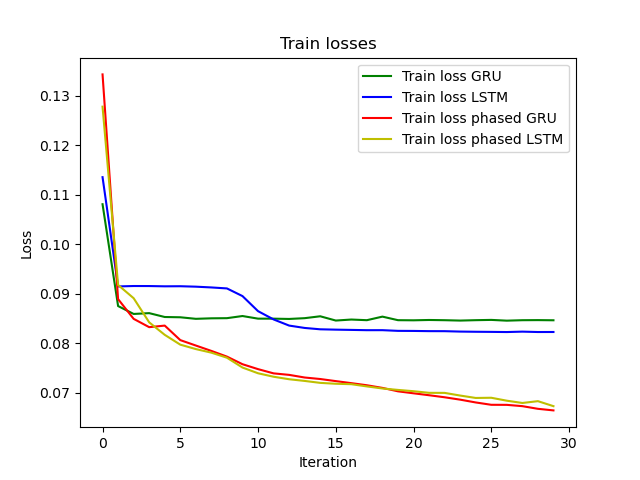
\includegraphics[height=10cm]{images/TrainingLosses_all.png}
\caption{Training losses}
\label{fig:trainloss}
\end{figure}
The training loss of the two models without time gate converges quickly after a few epochs the training error of the basic GRU model isn't changing significantly anymore, the training loss of the basic LSTM model does another significant jump down around the 10th epoch whereafter it remains pretty much constant and ends with a little lower loss than the GRU model. The time-gated models perform substantially better regarding the training loss. Not only do they end with a lower training loss, but after 30 epochs the loss still is decreasing for both models. \\
\begin{figure}[h] 
\centering
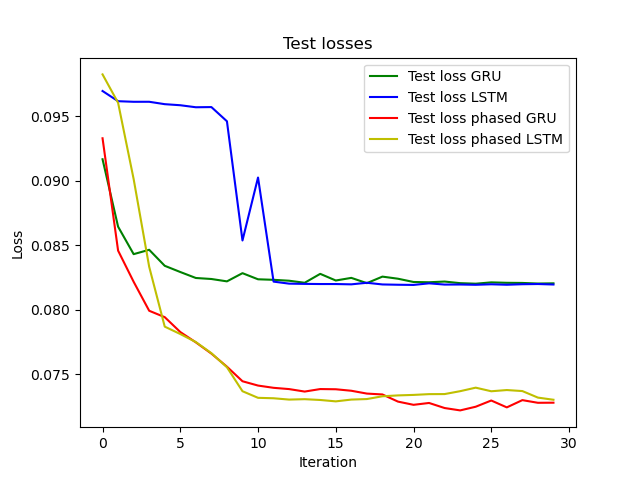
\includegraphics[height=10cm]{images/TestLosses_all.png}
\caption{Test losses}
\label{fig:testloss}
\end{figure}
\\
Similar development is displayed in the test loss. The networks with time gates perform notably better than the two models without. We see that the small jump in training error we observed in \ref{fig:trainloss} for the LSTM network around the 10th epoch corresponds to a huge decrease in test loss. 

Therefore we conclude a big effect of the time gate on the performance of the networks. 

All other metrics are calculated on the test data 
\begin{figure}[h]
\begin{minipage}[c]{0.5\linewidth}
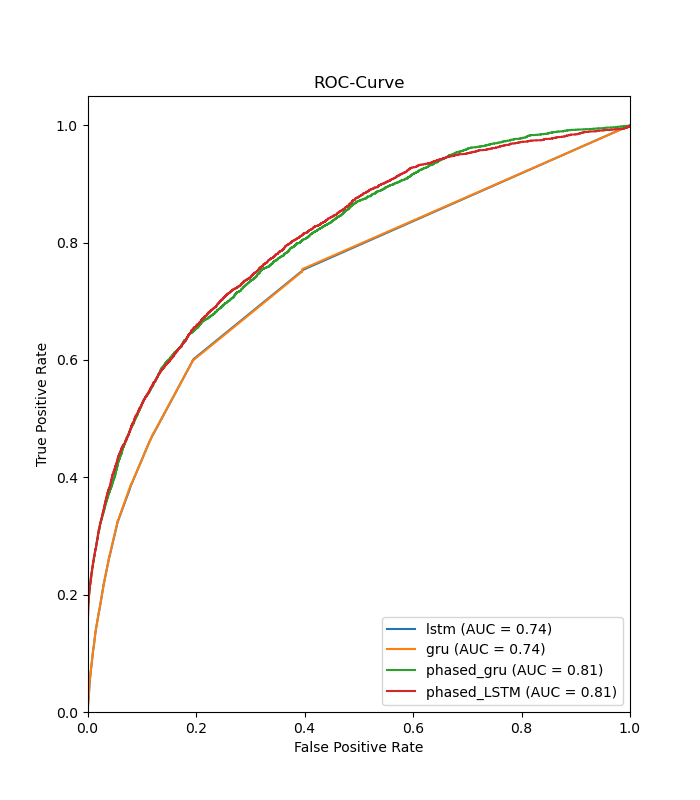
\includegraphics[width=\linewidth]{images/AUC_all.png}
\caption{ROC/AUC}
\label{fig:AUC}
\end{minipage}
\hfill
\begin{minipage}[c]{0.5\linewidth}
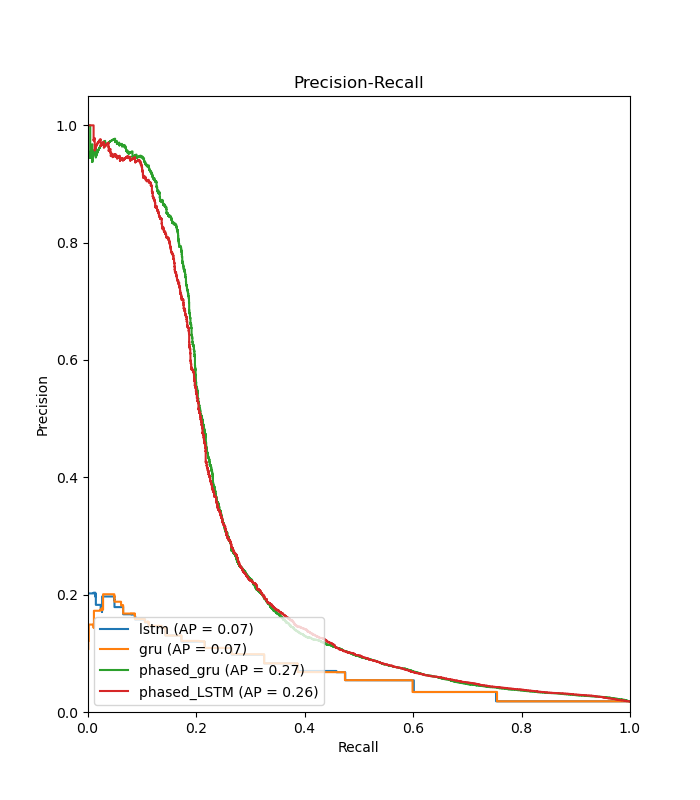
\includegraphics[width=\linewidth]{images/PR_all.png}
\caption{Precision Recall}
\label{fig:PR}
\end{minipage}%
\end{figure}


\begin{center}
\begin{tabular}{ |m{4cm}||m{2.5cm}|m{2.5cm}|m{2.5cm}|m{2.5cm}| } 
  \hline 
    & \textbf{phased GRU} & \textbf{GRU} & \textbf{phased LSTM} & \textbf{LSTM}\\ 
  \hline \hline
  trainable Parameters & \textbf{87,624} & 87,682 & 116,744 & 116,866 \\
  \hline
  Fitting time & 5011s &  \textbf{3910s} & 11808s & 5666s \\ 
  \hline
  Accuracy &  \textbf{0.98406} & 0.98178 & 0.98372 & 0.98178 \\ 
  \hline  
  Precision &  \textbf{0.78162} & - & 0.73281 & - \\ 
  \hline
  Recall & 0.17377 & - & 0.16726 & - \\ 
  \hline
  ROC-AUC & \textbf{0.81} & 0.74 &  \textbf{0.81} & 0.74 \\
  \hline  
  train loss &  0.06646 & 0.08467 & 0.06731 & {0.08230} \\ 
  \hline
  test loss &  \textbf{0.07277} & 0.08203  & 0.07300 & 0.08194 \\ 
  \hline
  minimal test loss &  \textbf{0.07218} & 0.08200 & 0.07287 & 0.08191 \\
  \hline
\end{tabular}
\end{center}



